\documentclass{article}
\usepackage{tikz}

% Use the maximum amount of space on a page
\textwidth=20cm
\textheight=28cm
\oddsidemargin=0pt
\topmargin=0pt
\headheight=0pt
\headsep=0pt

\newlength{\height}
\newlength{\width}
\newlength{\offset}

\setlength{\height}{2.4cm}  % Height of a square
\setlength{\width}{3cm}     % Width of a square
\setlength{\offset}{2.3cm}  % Offset of the squares from the shaded line

\begin{document}
\thispagestyle{empty}

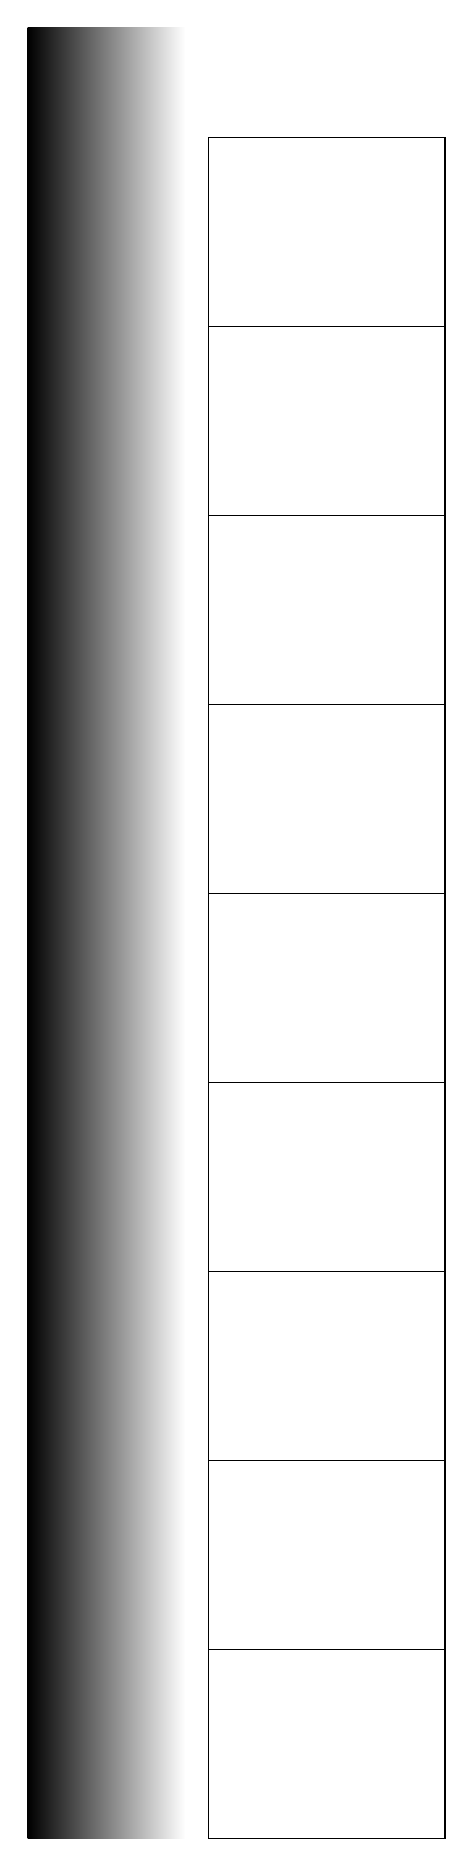
\begin{tikzpicture}
% Draw the gray gradient line 2cm x 23 cm
\shade[left color=black,right color=white] (0,0) rectangle +(2,23);

% Draw the white rectangles
\foreach \a in {0,...,8}
  \draw (\offset,\height*\a) rectangle +(\width,\height);
\end{tikzpicture}
\end{document}
